\clearpage
\section{Dark current}
All data used in this chapter are already taken beforehand and provided to us. Three images with \SI{30}{\s}, \SI{60}{\s}, and \SI{120}{\s} exposure times are taken at temperature between \SI{-10}{\degreeCelsius} and \SI{10}{\degreeCelsius} with step of \SI{2}{\degreeCelsius}. Raw data can be found in appendix~\ref{app:darkCurrent}.

Data with \verb|imstats| are taken in region $1800 < x < 2800, 300 < y < 800$. Mean of the images is chosen as the measure of dark current and bias. It might be influences by cosmic rays, random fluctuations and so on. But it also has variance (sigma) provided. Variance can be used further in curve fitting process. In the end, mode, mean and median don't differ from each other very much, if one looks at the raw data anyway.

For every temperature, a linear fitting is done to the three data points. Slope corresponds to dark current \textit{after} converted by gain. Intercept can be interpreted as bias level. These two quantities are plotted in figure~\ref{fig:darkCurrent},~\ref{fig:bias}.
\begin{figure}[ht]
	\centering
	\includegraphics[width=0.8\linewidth]{darkCurrent.pdf}
	\caption{Dark current. Obtained from slope of points at one temperature and then converted to in unit of $e^-$.}%
	\label{fig:darkCurrent}
\end{figure}
\begin{figure}[ht]
	\centering
	\includegraphics[width=0.8\linewidth]{bias.pdf}
	\caption{Bias from intercept of linear fitting}%
	\label{fig:bias}
\end{figure}

Since slope and intercept are calculated from the same fitting process, there are correlation between these two to some extent. For simplicity, correlations are ignored and only the diagonal entries of the covariance matrix are used in further discussion. Errors drawn in figure~\ref{fig:darkCurrent} and~\ref{fig:bias} are thus the diagonal part of the matrix. Dark current is here given in unit of \si{\ele\per\px\per\s}, thus we want to convert it using gain from later parts (section~\ref{sec:gain} and~\ref{sec:linear}). These two values are combined (averaged) and their errors are propagated properly (variance is additive). The gain used here is
\begin{equation*}
	k = \SI{1.49 +- 0.05}{\ele\per\ADU}
\end{equation*}
Error of dark current is given in
\begin{equation*}
	\sigma_{I_\text{dark}} = I_\text{dark} \sqrt{ \left( \frac{\sigma_k}{k} \right)^2 + \left( \frac{\sigma_{I_{\text{dark,d}}}}{I_{\text{dark,d}}} \right)^2  }	
\end{equation*}

In figure~\ref{fig:bias}, bias levels somewhat depend on the temperature as well. This might be understood because the determined dark current and bias have correlation in the fitting process. Or maybe the cooling also affects the read-out circuit. Anyway this fluctuation is really tiny ($\sim 0.2\%$).

The fit curve in figure~\ref{fig:darkCurrent} is done with equation~\ref{Equ:DarkCurrent}, but with extra additive constant $A$. This constant makes the fitting so much better. The origin of this constant is still puzzle to us. With it, dark current at quite low temperature could be negative, thus the model breaks down. These parameters are
\begin{align*}
	c &= \SI{1516853.877 +- 90255.383}{\ele\per\px\per\s\kelvin\tothe{-3/2}} \\
	A &= \SI{-0.030 +- 0.005}{\ele\per\px\per\s}
\end{align*}
Expected dark current at $T=\SI{-25}{\degreeCelsius}$ would be
\begin{equation*}
	I_\text{dark} (T = \SI{-25}{\degreeCelsius}) = \SI{-0.030 +- 1.035}{\ele\per\px\per\s}
\end{equation*}
This amount of dark current would not affect image quality in HOLIGRAIL observations too much. An exemplar science frame has exposure time of \SI{300}{\s} and then noise due to dark current would be about \SI{6}{\ADU}. This is negligible since the "background" of the science has typically $\sim \SI{600}{\ADU}$ and bias has something like $\sim \SI{200}{\ADU}$.

In figure~\ref{fig:bias} and~\ref{fig:darkCurrent}, one might see the x-axis is the set temperature instead of real temperature. Quite understandable there are some fluctuations around the set temperature, since the temperature control circuit/chip cannot be perfect. These fluctuations are not taken in consideration while doing the (first set of) curve fits to find dark current. By doing this the errors are not underestimated, since these fluctuations would also influence the pixel values at different exposure times. It will leads to (usually) larger uncertainties in dark current and bias. One could try to use model function with the determined parameters to correct the temperatures to the set values. But it would not be necessary and potentially problematic, because the data might have some bias towards the existing parameters.

\section{Detector system "gain" and noise}\label{sec:gain}
For this part, one bias and two flats are provided. In order to get rid of the PRNU noise, a difference frame of these two flats is generated with the command \verb|ic| provided in~\cite{manual}.

Bias frame contains only the RON, since it is not exposed to light. Difference frame only have RON and photon noise
\begin{equation*}
	\sigma^2_\text{diff, d} = 2\sigma^2_\text{RON, d} + 2\sigma^2_{e, \text{d}}
\end{equation*}
The factor $2$ arises because the variance is additive when calculating difference of two images. Then one can subtract the RON from bias frame to extract the photon noise
\begin{equation}
	\sigma_{e, \text{d}} = \SI{144.81}{\ADU}
\end{equation}

In principle, PRNU noise can be extracted in the same way, whereas we have here two flat images. Thus signal levels of two images get averaged (one can obtain an error estimate by the way) and their variance as well according to propagation of uncertainties
\begin{align*}
	N_{e, \text{d}} &= \SI{31742.94 +- 7.85}{\ADU} \\
	\sigma_\text{flats, d} &= \frac{1}{2} \sqrt{\sigma^2_{\text{flat, d}, 1} + \sigma^2_{\text{flat, d}, 2}}
\end{align*}
Subtracting two previous computed noises, we have the PRNU noise
\begin{equation}
	\sigma_\text{PRNU, d} = \SI{140.38}{\ADU}	
\end{equation}
With equation~\ref{math:fPRNU},
\begin{equation}
	f_\text{PRNU} = (\num{4.422 +- 0.001}) \cdot 10^{-3}
\end{equation}
This has similar order of magnitude as given in~\cite{manual}.

One could determine the gain with the help of equation~\ref{math:gain}. It is
\begin{equation}
	k = \SI{1.514 +- 0.000}{\ele\per\ADU}
\end{equation}
As a reference, the RON noise in unit of electron is
\begin{equation}
	\sigma_\text{RON} = \SI{14.881 +- 0.004}{\ele}
\end{equation}

\section{Detector linearity and full-well capacity}\label{sec:linear}
Again, the data are already taken and we assume that these images are ordered randomly to avoid systematic effects. These images are taken with red filter and the set temperature is \SI{-10}{\degreeCelsius}. The signal level and other informations are evaluated in a uniformly illuminated region: $1200 < x < 1600$ and $400 < y < 600$. Raw data can be found in appendix~\ref{app:detLinear}.

Once pixels in CCD get saturated, pixel count increase non-linearly. This can be easily seen in signal level against exposure time plot, see figure~\ref{fig:exp_mean}. Signal level refers to the mean pixel counts in the image. Here the fitting is done only to the points roughly on a straight line. This line is described by
\begin{equation}
	S(t) = a\cdot t + b =  \SI{61097.242}{\ADU \per\s} \cdot t + \num{2091.783}
	\label{math:ft}
\end{equation}
\begin{figure}[ht]
	\centering
	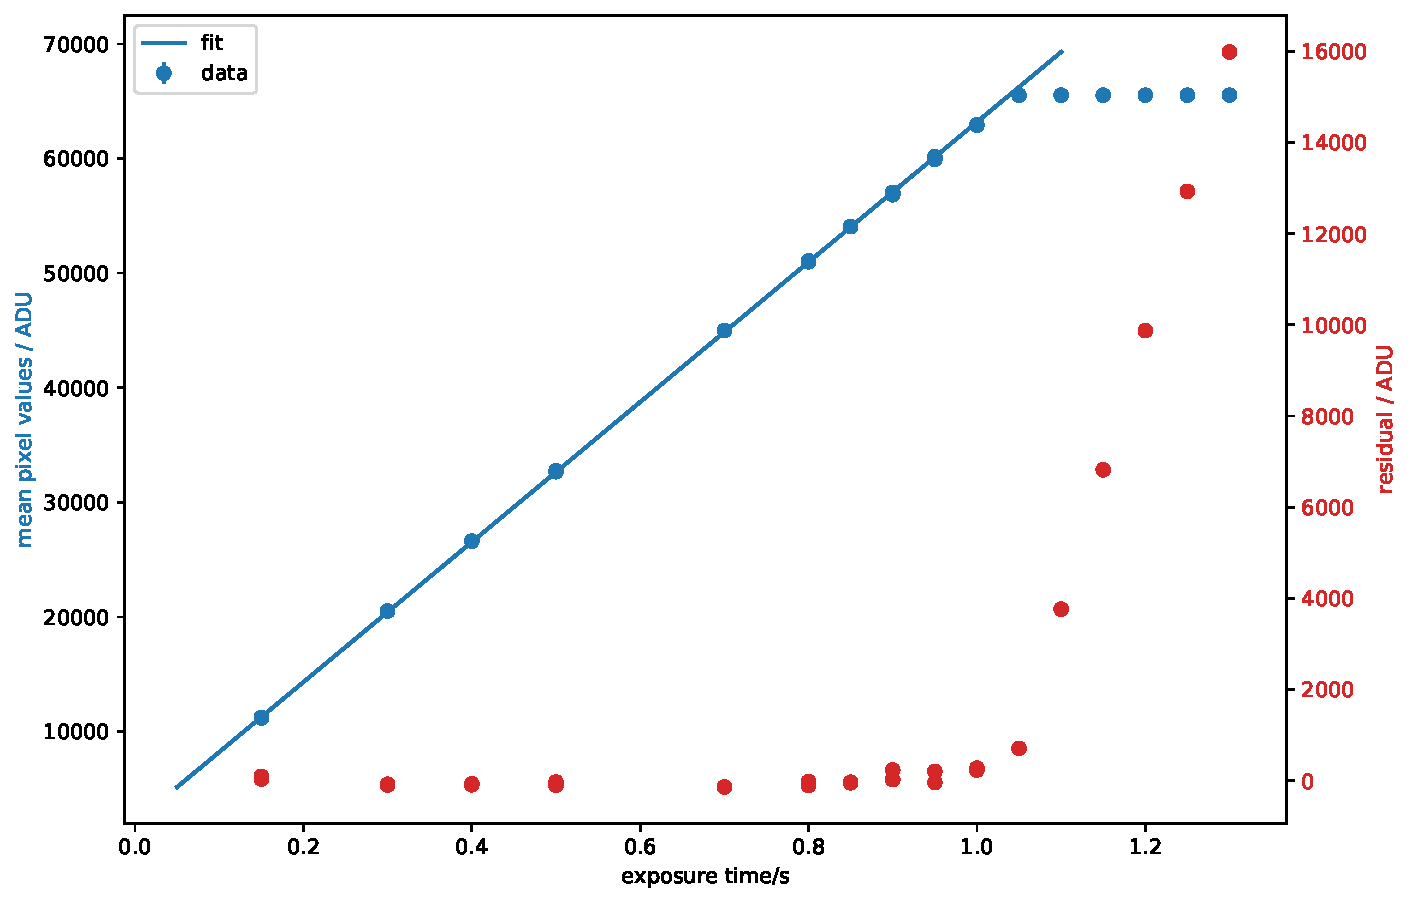
\includegraphics[width=0.8\linewidth]{exp_mean.pdf}
	\caption{Signal level (mean) against exposure time and residuals.}%
	\label{fig:exp_mean}
\end{figure}

Using this expression we can calculated exposure time given some signal levels.
Covariance matrix (of the fit parameters) is 
\begin{equation*}
	\Sigma_{ab} =  \begin{pmatrix} 6917.573 & -2829.764 \\ -2829.764 & 1702.991 \end{pmatrix}
\end{equation*}
Clearly this matrix is not (loosely) diagonal, thus the parameters are somewhat correlated. Inverting the function in equation~\ref{math:ft} gives us a non-linear function in parameters $a$ and $b$. Nonetheless, one could just the mighty Taylor expansion and use the Jacobian to try to propagate the errors
\begin{equation}
	\Sigma_t = J \Sigma_{ab} J^T
	\label{math:Sigma}
\end{equation}
Maximal exposure time without saturation can be computed using \ref{math:ft}, its error using~\ref{math:Sigma}. Non-linearity kicks in at exposure time of \SI{1.034}{\second}. The error is really tiny at $\num{8.8} \cdot 10^{-7} \si{\s}$.

In fact, this determination can be improved by looking into difference frames of images with identical exposure time. Two frames with identical exposure time are recorded and get subtracted. The variance (or sigma) in difference frame will drop significantly, as soon as CCD gets saturated. So in principle, one can determine the maximal exposure time without saturation more precisely. \begin{figure}[ht]
	\centering
	\includegraphics[width=0.8\linewidth]{diff.pdf}
	\caption{Sigma against signal levels in log-log scale. At large exposure time, CCD gets fully saturated, thus the sigma is zero and corresponding data points cannot show up in log scale. Errors of signal level are taken as the sigma of the respective image, but not visible here.}%
	\label{fig:diff}
\end{figure}

In figure~\ref{fig:diff}, this drop is not so obvious, since after the steady climb the variance of difference frame goes to zero immediately. We claim that after the last point in figure~\ref{fig:diff} is where CCD gets saturated. Just as a rough estimate, saturation level is calculates as the mean value of the last point shown in figure~\ref{fig:diff} and its next point (with zero variance) and error is taken as the distance to each of these two points: $\SI{64233. 35+- 2599.89}{\ADU}$.

The straight line (at least in normal scale) is parameterized as
\begin{equation*}
	\sigma^2 (N) = a\cdot N + b = \SI{1.36}{\ADU} \cdot N + (\SI{-1038.89}{\ADU\tothe{2}})
\end{equation*}
with covariance matrix
\begin{equation}
	\sigma_{ab} = \begin{pmatrix}  \num{1.78e-3} & \num{75.13} \\ \num{-75.13} & \num{3.69e6}\end{pmatrix}
\end{equation}

The slope can be used to compute the gain $k$ using equation~\ref{math:gain}. Unfortunately, real life is complicated as always. The pixel value of the difference frame is a linear combination of individual frames (difference). Thus the variance simply add with each other. Here the fixed pattern noise is irrelevant, since it doesn't vary between exposures. Thus the pixel value of difference frame will only contain statistical error (photon noise). We have now
\begin{equation}
	k = \frac{N_{e,d}}{ \sigma^2_{\text{diff}}/2}
\end{equation}
Thus the slope of the line is $\frac{2}{k}$. Assuming that the fit parameters are uncorrelated and we just take the diagonal entries as the uncertainty for the slope. The gain is determined to be
\begin{equation}
	k = (\num{1.47 +- 0.05} ) e^{-}\si{\per\ADU}
\end{equation}
Its error is propagated with
\begin{equation*}
	\sigma_k = \left| \frac{2}{a^2} \sigma_a \right|
\end{equation*}

With the value of gain, saturation value can be converted to in units of $e^{-}$, i.e.~full-well capacity
\begin{equation}
	\text{full-well} = (\num{94479.66 +- 4820.67}) e^-
\end{equation}
where the error is computed by
\begin{equation*}
	\sigma^2_\text{fw} = \text{fw} \cdot \sqrt{(\sigma_k/k)^2 + (\sigma_\text{sat}/\text{sat})^2}
\end{equation*}
